La persistencia de datos es muy importante de cara a mantener una aplicación web. Sin embargo, en los marcos de trabajo actuales, es habitual descargar mucha carga de datos en el cliente y que este lo vaya administrando. Esta gestión puede ser muy tediosa si no se utilizan unas tecnologías llamadas capas de datos, que permiten mantener la coherencia de los datos en toda la aplicación. Las herramientas más populares se muestran en la Figura \cref{fig:stjs2019:datalayer}. 

Se puede apreciar que GraphQL es líder en este sector, y no por pocos motivos. Esta herramienta fue creada por Facebook (al igual que React y su principal competidora, Redux) y ha nacido a raíz de algunos problemas que surgían al utilizar React. Sin embargo, no está diseñada exclusivamente para React. GraphQL se puede utilizar junto con cualquier entorno. Dado que esta herramienta es la más popular en el mercado, está diseñada por los creadores de React y resuelve los problemas que explica \citet{RDXVGQL} en su artículo, es la herramienta elegida para el marco que se ha desarrollado.

Sin embargo, no siempre se necesita capa de datos en el cliente y, por tanto, la posibilidad de utilizar GraphQL será una configuración opcional. En la configuración inicial, al desarrollador se le preguntará si desea capa de datos (GraphQL) en su entorno y este podrá sencillamente contestar si lo desea o prefiere desarrollar su producto controlando la capa de datos de forma personalizada, ya sea mediante otra herramienta o cuidando el estado y las propiedades de sus componentes de React.

\begin{figure}
	\centering
	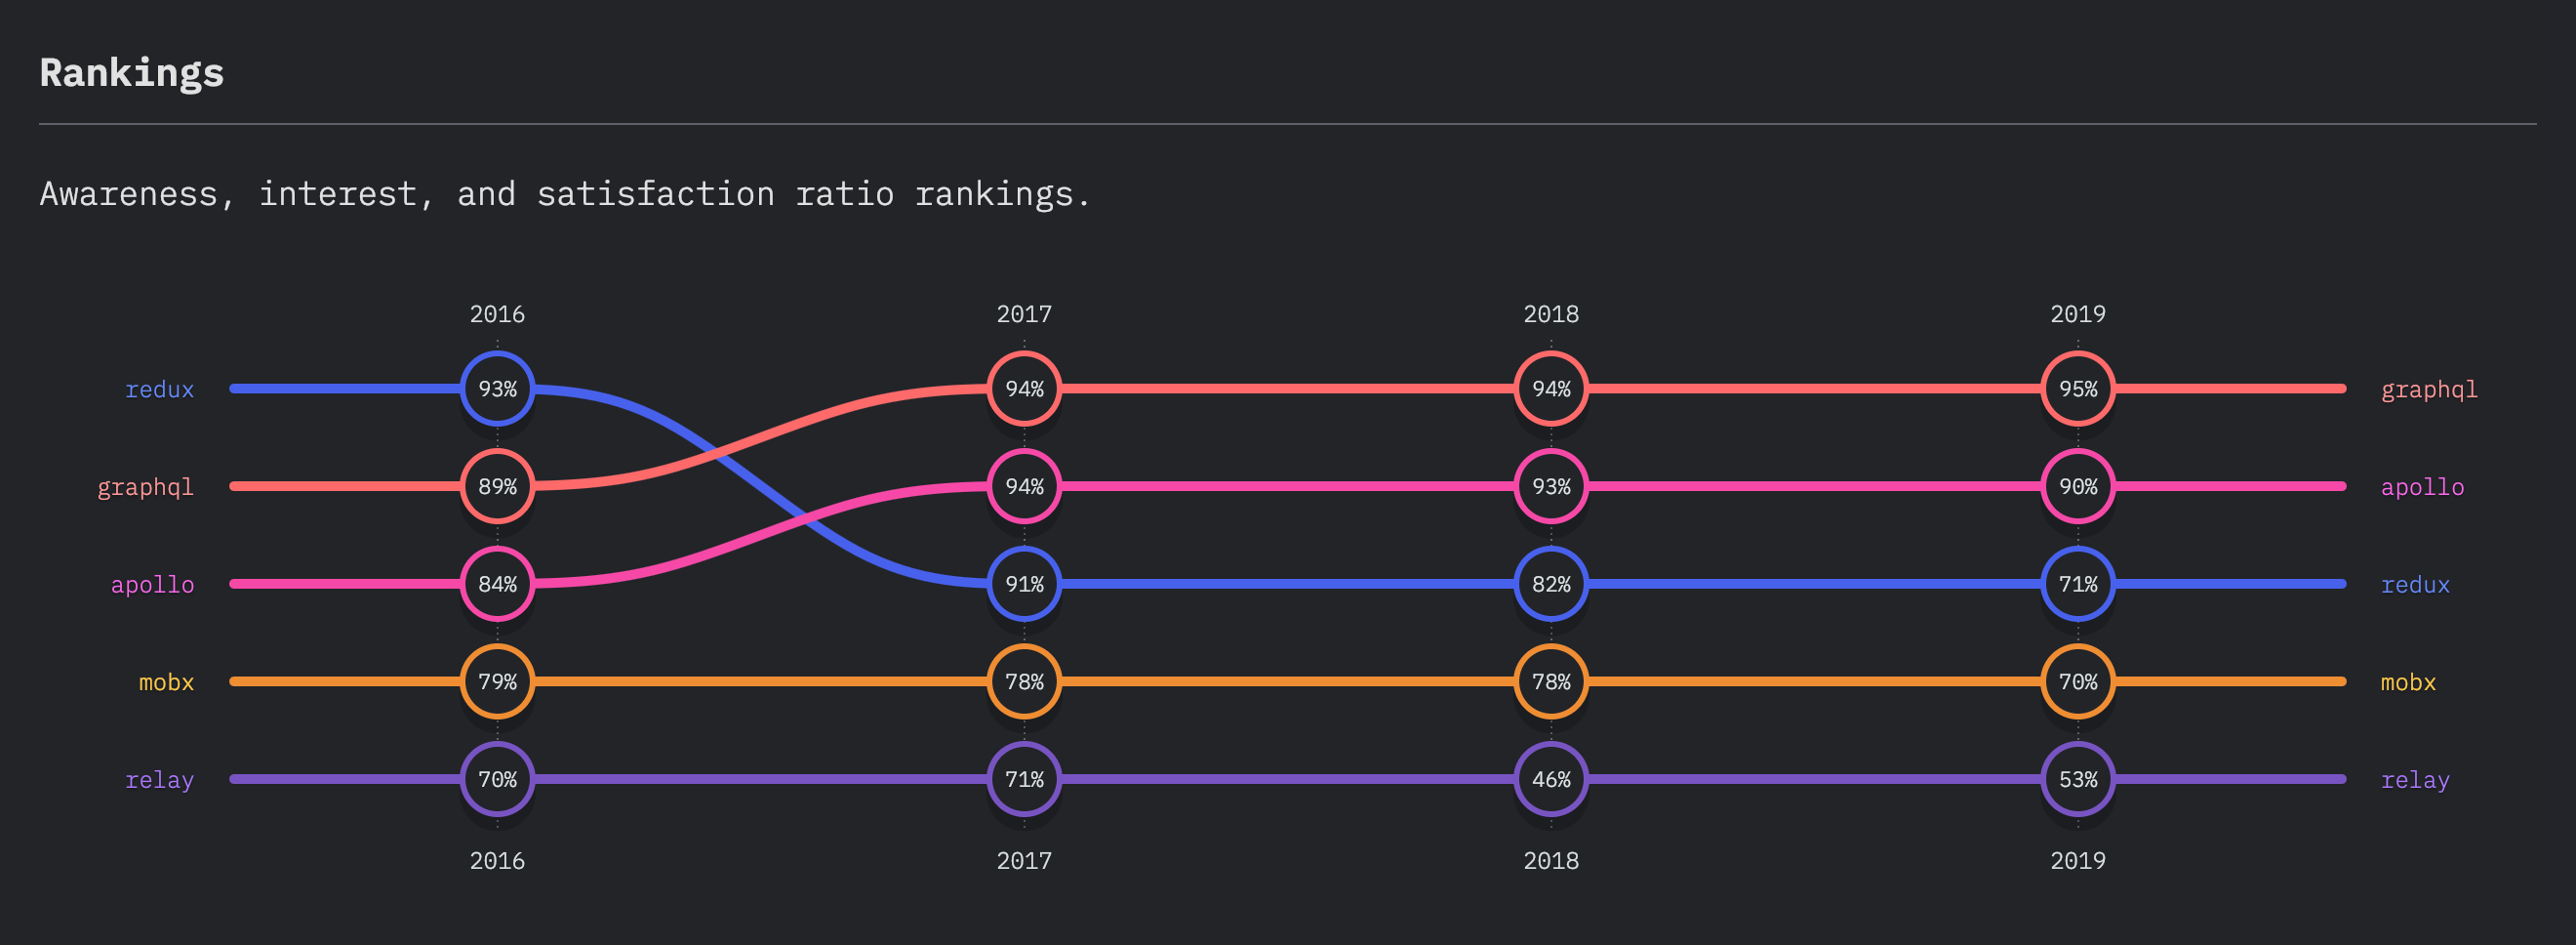
\includegraphics[width=\textwidth]{data_layer_popularity.png}
	\caption{2019 - Opinión popular de las herramientas de gestión de la capa de datos}
	\label{fig:stjs2019:datalayer}
\end{figure}
